\section{Payload}
\label{sec:payload}

\uH's payload is part of STS1 (SpaceTeamSat1), a different TU Wien Space Team project. SpaceTeamSat1 is a 1U cubesat, its primary mission is to design and build a cubesat completely in-house that will eventually fly orbit in space and survive the conditions there. The secondary mission of STS1 is to give students the opportunity to run their own Python scripts in space. The scripts are executed on a Raspberry PI CM 3+, which is connected to several sensors via an I2C bus. The sensors include temperature, magnet, gas, acceleration and more.

\begin{figure}
    \centering
    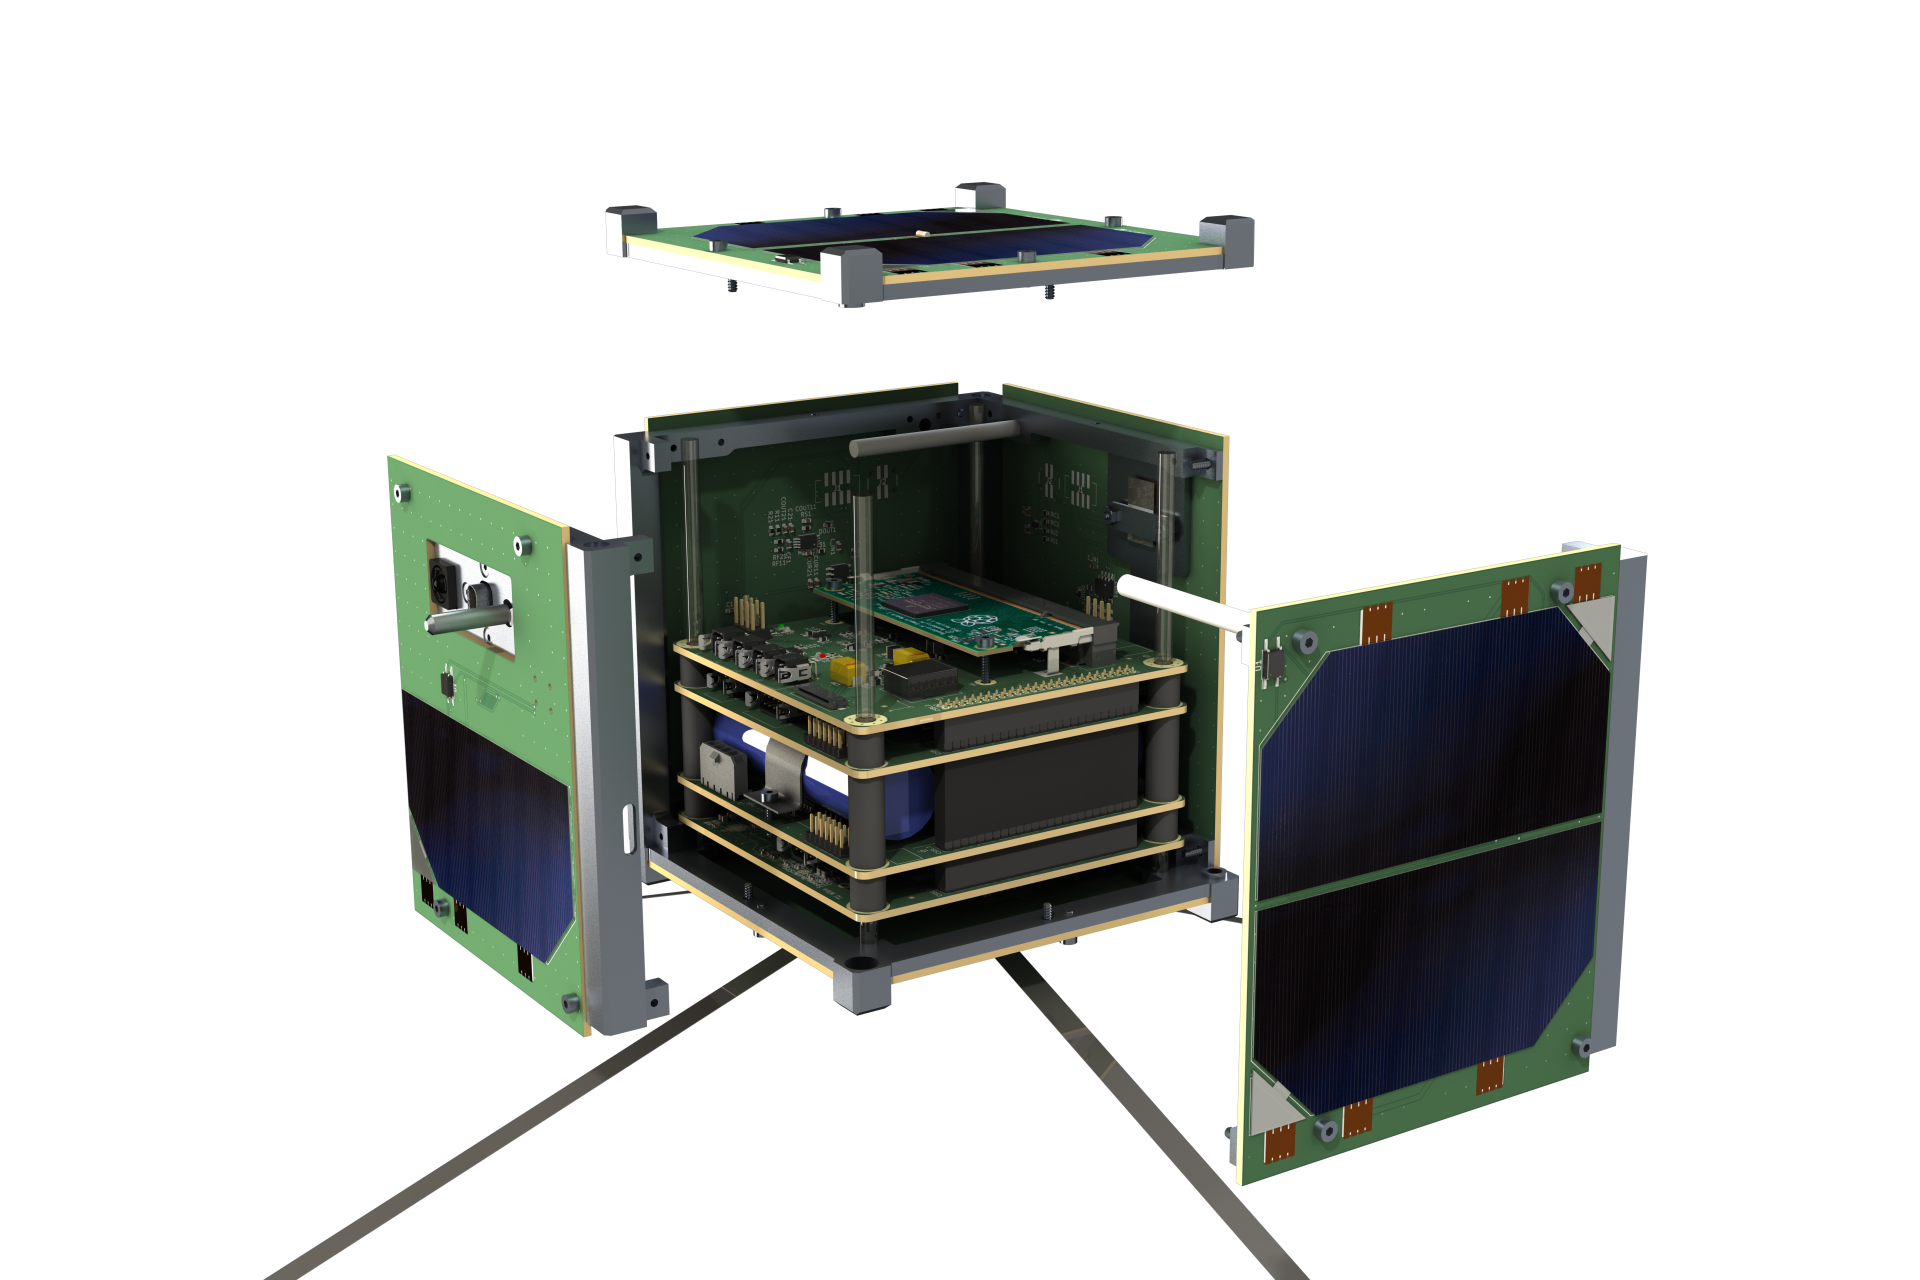
\includegraphics[width=0.7\textwidth]{Payload/STS1_Payload.png}
    \caption{Payload: STS1 Render}
    \label{fig:payload_render}
\end{figure}

This inter-project collaboration offered itself as the \uH launch is a great opportunity to flight test some of the hardware for the cubesat and because \uH needs to fly a payload anyways. Since the full 1U cubesat wouldn't fit inside the \uH airframe only the EDU subsystem is going to be flown.

To fulfill the internal goals for the payload the education subsystem of STS1 and a power supply is required. The whole assembly is installed in a \SI{100}{\milli\meter} x \SI{100}{\milli\meter} x \SI{50}{\milli\meter} housing with a total mass of \SI{1}{\kilogram}, this meets the requirement of four PocketSats with a mass of \SI{250}{\gram} each.